\section{Graph Characterization of Partial Views}\label{sec:graph-characterization}
%==============================================================================


Before defining the general confusability graph, we develop a concrete example: partial observations can induce nontrivial failure topology.

\begin{figure}[t]
\centering
\ifdefined\ITSUBMISSION
  \resizebox{0.9\textwidth}{!}{%
  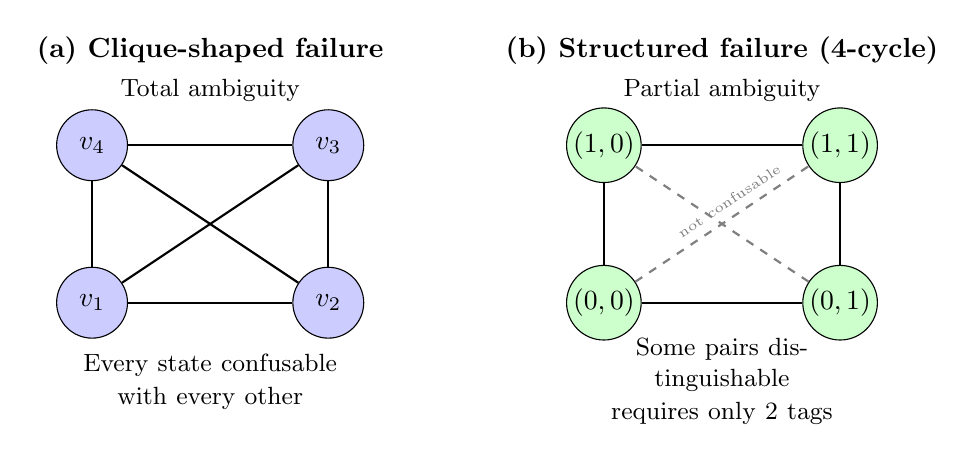
\begin{tikzpicture}
    % Panel A: Clique
    \begin{scope}[xshift=0cm, yshift=-1.2cm]
      \node at (1.5, 3.2) {\textbf{(a) Clique-shaped failure}};
      \node at (1.5, 2.7) {\small Total ambiguity};

      % Four vertices in a square
      \node[circle, draw, fill=blue!20, minimum size=9mm, inner sep=1pt] (a1) at (0, 0) {$v_1$};
      \node[circle, draw, fill=blue!20, minimum size=9mm, inner sep=1pt] (a2) at (3, 0) {$v_2$};
      \node[circle, draw, fill=blue!20, minimum size=9mm, inner sep=1pt] (a3) at (3, 2) {$v_3$};
      \node[circle, draw, fill=blue!20, minimum size=9mm, inner sep=1pt] (a4) at (0, 2) {$v_4$};

      % All edges (clique)
      \draw[thick] (a1) -- (a2) -- (a3) -- (a4) -- (a1);
      \draw[thick] (a1) -- (a3);
      \draw[thick] (a2) -- (a4);

      \node[text width=3.5cm, align=center] at (1.5, -1.0) {\small Every state confusable\\with every other};
    \end{scope}

    % Panel B: 4-cycle
    \begin{scope}[xshift=6.5cm, yshift=-1.2cm]
      \node at (1.5, 3.2) {\textbf{(b) Structured failure (4-cycle)}};
      \node at (1.5, 2.7) {\small Partial ambiguity};

      % Four vertices in a square
      \node[circle, draw, fill=green!20, minimum size=9mm, inner sep=1pt] (b1) at (0, 0) {$(0,0)$};
      \node[circle, draw, fill=green!20, minimum size=9mm, inner sep=1pt] (b2) at (3, 0) {$(0,1)$};
      \node[circle, draw, fill=green!20, minimum size=9mm, inner sep=1pt] (b3) at (3, 2) {$(1,1)$};
      \node[circle, draw, fill=green!20, minimum size=9mm, inner sep=1pt] (b4) at (0, 2) {$(1,0)$};

      % Cycle edges only
      \draw[thick] (b1) -- (b2);
      \draw[thick] (b2) -- (b3);
      \draw[thick] (b3) -- (b4);
      \draw[thick] (b4) -- (b1);

      % Dashed lines for non-edges
      \draw[dashed, gray, thick] (b1) -- (b3) node[pos=0.59, above, sloped, font=\tiny] {not confusable};
      \draw[dashed, gray, thick] (b2) -- (b4);

      \node[text width=3.5cm, align=center] at (1.5, -1.0) {\small Some pairs distinguishable\\requires only 2 tags};
    \end{scope}
  \end{tikzpicture}%
  }%
\else
  \resizebox{0.48\textwidth}{!}{%
  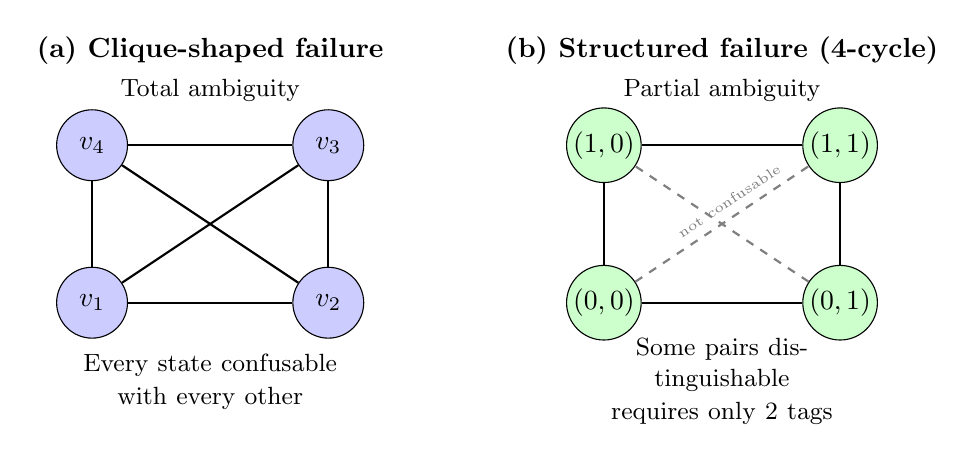
\begin{tikzpicture}
    % Panel A: Clique
    \begin{scope}[xshift=0cm, yshift=-1.2cm]
      \node at (1.5, 3.2) {\textbf{(a) Clique-shaped failure}};
      \node at (1.5, 2.7) {\small Total ambiguity};

      % Four vertices in a square
      \node[circle, draw, fill=blue!20, minimum size=9mm, inner sep=1pt] (a1) at (0, 0) {$v_1$};
      \node[circle, draw, fill=blue!20, minimum size=9mm, inner sep=1pt] (a2) at (3, 0) {$v_2$};
      \node[circle, draw, fill=blue!20, minimum size=9mm, inner sep=1pt] (a3) at (3, 2) {$v_3$};
      \node[circle, draw, fill=blue!20, minimum size=9mm, inner sep=1pt] (a4) at (0, 2) {$v_4$};

      % All edges (clique)
      \draw[thick] (a1) -- (a2) -- (a3) -- (a4) -- (a1);
      \draw[thick] (a1) -- (a3);
      \draw[thick] (a2) -- (a4);

      \node[text width=3.5cm, align=center] at (1.5, -1.0) {\small Every state confusable\\with every other};
    \end{scope}

    % Panel B: 4-cycle
    \begin{scope}[xshift=6.5cm, yshift=-1.2cm]
      \node at (1.5, 3.2) {\textbf{(b) Structured failure (4-cycle)}};
      \node at (1.5, 2.7) {\small Partial ambiguity};

      % Four vertices in a square
      \node[circle, draw, fill=green!20, minimum size=9mm, inner sep=1pt] (b1) at (0, 0) {$(0,0)$};
      \node[circle, draw, fill=green!20, minimum size=9mm, inner sep=1pt] (b2) at (3, 0) {$(0,1)$};
      \node[circle, draw, fill=green!20, minimum size=9mm, inner sep=1pt] (b3) at (3, 2) {$(1,1)$};
      \node[circle, draw, fill=green!20, minimum size=9mm, inner sep=1pt] (b4) at (0, 2) {$(1,0)$};

      % Cycle edges only
      \draw[thick] (b1) -- (b2);
      \draw[thick] (b2) -- (b3);
      \draw[thick] (b3) -- (b4);
      \draw[thick] (b4) -- (b1);

      % Dashed lines for non-edges
      \draw[dashed, gray, thick] (b1) -- (b3) node[pos=0.59, above, sloped, font=\tiny] {not confusable};
      \draw[dashed, gray, thick] (b2) -- (b4);

      \node[text width=3.5cm, align=center] at (1.5, -1.0) {\small Some pairs distinguishable\\requires only 2 tags};
    \end{scope}
  \end{tikzpicture}%
  }%
\fi
\caption{Two failure topologies. In (a), the observation provides no discrimination, so the confusability graph is a clique: every state is confusable with every other, and exact recovery requires a tag for each state. In (b), partial observations provide some discrimination: opposite corners are distinguishable even though adjacent states are not. The 4-cycle is 2-colorable, so exact recovery requires only 2 tags. This structural difference is invisible to the unit-rate threshold alone.}
\label{fig:failure-topology}
\end{figure}

\subsection{A Running Example: The Binary Square}\label{sec:binary-square}

Consider a system with two binary facts $(x_1, x_2) \in \{0,1\}^2$, giving four latent states:
\[
(0,0), \quad (0,1), \quad (1,0), \quad (1,1).
\]
View 1 reveals $x_1$ and View 2 reveals $x_2$.

\paragraph{Confusability structure.}
Two states are confusable when at least one view fails to separate them. View 1 reveals $x_1$, so $(0,0)\sim(0,1)$ and $(1,0)\sim(1,1)$. View 2 reveals $x_2$, so $(0,0)\sim(1,0)$ and $(0,1)\sim(1,1)$. The confusability graph is therefore a 4-cycle:
\[
(0,0) \sim (0,1) \sim (1,1) \sim (1,0) \sim (0,0),
\]
where opposite corners are not adjacent.

\paragraph{Exact recovery.}
The graph is 2-colorable (e.g., color by parity $c(x_1,x_2) = x_1 \oplus x_2$), so exact recovery is possible with a 2-ary auxiliary tag. With one tag, the best exact success probability under the uniform source is $1/2$.

\noindent\textbf{Coding-theoretic interpretation.} The parity coloring $c(x_1,x_2)=x_1\oplus x_2$ is a syndrome bit: with $T=2$ we decode perfectly, with $T=1$ we cannot distinguish adjacent vertices. The confusability graph is the confusion graph of a code with parity-check $H=[1\;1]$.

Figure~\ref{fig:failure-topology} contrasts this structured failure with clique-shaped failure. The theorems below generalize this to arbitrary multi-fact partial-view systems.

\subsection{General Graph Characterization}

\begin{definition}[Coordinate-Subset View]\label{def:coordinate-view}
For a $d$-fact latent tuple $x=(x_1,\dots,x_d)$ and a coordinate set $S\subseteq[d]$, the \emph{coordinate-subset view} indexed by $S$ is the projection
\[
\pi_S(x) := x|_S.
\]
\end{definition}

\begin{definition}[Admissible View Family]\label{def:admissible-view-family}
An \emph{admissible view family} is a finite family $\mathcal V=\{V_1,\dots,V_m\}$ of coordinate subsets of $[d]$, where view $V_\ell$ reveals exactly the coordinates indexed by $V_\ell$.
\end{definition}

\begin{definition}[Agreement Set]\label{def:agreement-set}
For latent tuples $x,y\in\mathcal X$, their \emph{agreement set} is
\[
\operatorname{Agr}(x,y) := \{i\in[d] : x_i = y_i\}.
\]
\end{definition}

\begin{definition}[Upward-Closed Family]\label{def:upward-closed-family}
A family $\mathcal U\subseteq 2^{[d]}$ is \emph{upward-closed} if whenever $S\in\mathcal U$ and $S\subseteq T\subseteq[d]$, one also has $T\in\mathcal U$.
\end{definition}

\begin{definition}[Confusability Graph]\label{def:confusability-graph}
Given latent state space $\mathcal X$ and admissible view family $\mathcal V$, the \emph{confusability graph} is the graph
\[
G_{\mathrm{conf}}=(\mathcal X,E_{\mathrm{conf}})
\]
whose vertices are the latent states and whose edges are the unordered pairs $\{x,y\}$ with $x\neq y$ for which there exists an admissible view $V_\ell\in\mathcal V$ such that $\pi_{V_\ell}(x)=\pi_{V_\ell}(y)$. Equivalently, $\{x,y\}\in E_{\mathrm{conf}}$ iff some admissible view is contained in $\operatorname{Agr}(x,y)$.
\end{definition}

\begin{definition}[Confusability Oracle]\label{def:confusability-oracle}
The \emph{confusability oracle} is the Boolean adjacency test
\[
\mathsf{Conf}(x,y)=\mathbf 1\big[\{x,y\}\in E_{\mathrm{conf}}\big].
\]
\end{definition}

\begin{definition}[Agreement-Set Oracle]\label{def:agreement-set-oracle}
The \emph{agreement-set oracle} returns $\operatorname{Agr}(x,y)$. In the coordinate-view model, one may decide confusability by computing $\operatorname{Agr}(x,y)$ and testing whether some admissible view is contained in it.
\end{definition}

For $d$ facts over alphabet size $q$, explicit graph materialization has $q^d$ vertices and at most $q^{2d}$ ordered state pairs, but adjacency is available through the confusability oracle or the equivalent agreement-set oracle. The oracle computation takes $O(d + \sum_{\ell}|V_\ell|)$ time by computing the agreement set and scanning the admissible views.\leanmeta{\LHrng{MFT}{113}{117}, \LHrng{MFT}{132}{135}}

The Lean development also formalizes a support-overlap extension in which each location may emit any observation from a finite support set, and two states are confusable when some admissible location has overlapping support on those states.\leanmeta{\LHrng{MFT}{110}{112}}

In the exact coordinate-view model, confusability depends only on agreement sets. From any admissible view family we obtain the upward-closed family
\[
\mathcal U := \{S \subseteq [d] : \exists \ell,\; V_\ell \subseteq S\},
\]
and two distinct tuples are adjacent if and only if their agreement set lies in $\mathcal U$. Conversely, every upward-closed family arises from some coordinate-view architecture. When the alphabet has at least two symbols, every proper coordinate subset occurs as the agreement set of some distinct pair of tuples, and coordinatewise alphabet permutations preserve confusability and induce graph automorphisms.\leanmeta{\LHrng{MFT}{118}{131}}

\leanmetapending{\LHrng{MFT}{3}{4}, \LH{MFT20}}
\begin{theorem}[Exact recovery as graph colorability]\label{thm:multifact-colorability}
For a finite multi-fact latent tuple observed through a finite family of partial-coordinate views, exact zero-error recovery with a $T$-ary auxiliary tag exists if and only if the induced confusability graph is $T$-colorable~\cite{west2001introduction,diestel2017graph}.
\end{theorem}

\begin{proof}
Let $G_{\mathrm{conf}}$ be the confusability graph.

\emph{Necessity.} Suppose exact recovery with $T$ tags is possible. If two latent tuples are adjacent in $G_{\mathrm{conf}}$, then by definition some allowed observation leaves them indistinguishable. Exact recovery therefore cannot assign them the same tag, because the joint observation-tag pair would then coincide on two distinct latent tuples and Theorem~\ref{thm:pair-injective} would be violated. Hence the tag assignment is a proper $T$-coloring of $G_{\mathrm{conf}}$.

\emph{Sufficiency.} Suppose $c$ is a proper $T$-coloring of $G_{\mathrm{conf}}$. Define the auxiliary tag of a latent tuple to be its color. If two latent tuples produce the same observation and the same color, then they are confusable and adjacent, contradicting proper colorability. Therefore the joint observation-color map is injective, and Theorem~\ref{thm:pair-injective} yields an exact decoder.
\end{proof}

For repeated copies, the full block confusability graph is identified with the $n$-fold strong power of the one-shot confusability graph.\leanmeta{\LHrng{MFT}{34}{35}}

\leanmetapending{\LH{MFT9}}
\begin{theorem}[Success-set characterization]\label{thm:multifact-success-set}
In the same model, exact decoding on a designated success set $S$ is equivalent to $T$-colorability of the induced confusability subgraph on $S$.
\end{theorem}

\begin{proof}
Restrict the argument of Theorem~\ref{thm:multifact-colorability} to the success set. Exactness is required only on $S$, so the coloring condition is required only on confusable pairs inside $S$.
\end{proof}

\leanmetapending{\LHrng{MFT}{14}{15}}
\begin{theorem}[Exact finite-error success budget]\label{thm:multifact-max-success}
For each tag alphabet size $T>0$, there is a largest success-set size
\[
M_T := \max\{|S| : S \text{ induces a $T$-colorable subgraph}\}.
\]
An exact decoder with $T$ tags exists on a success set $S$ if and only if $|S|\le M_T$ after replacing $S$ by some $T$-colorable success set of size $M_T$. Under the uniform source, the optimal exact success probability is therefore $M_T/|\mathcal X|$.
\end{theorem}

\begin{proof}
Theorem~\ref{thm:multifact-success-set} identifies exact success sets with induced $T$-colorable subgraphs. Since the latent alphabet is finite, a maximum-cardinality such set exists. The mechanized characterization exposes this optimum directly. In the binary four-cycle witness, the optimum at $T=1$ is exactly two states, so the best uniform exact success probability is $2/4=1/2$.
\end{proof}

The same characterization is also available in weighted form. For any finite source weight $w$ on the latent alphabet, the maximum mass of a $T$-colorable induced subgraph is the exact finite success value under budget $T$.\leanmeta{\LHrng{MFT}{18}{19}, \LHrng{MFT}{23}{24}}

\leanmetapending{\LHrng{MFT}{5}{8}, \LH{MFT10}}
\begin{theorem}[First non-clique witness]\label{thm:multifact-nonclique}
There exists a binary two-fact system with single-coordinate observation views whose confusability graph is not a clique. In that system, two tags suffice for exact recovery, one tag is impossible, and any one-tag decoder can be exact on at most half of the four latent states under the uniform source.
\end{theorem}

\begin{proof}
The witness is the four-state binary square with one location revealing the first coordinate and the other revealing the second. States that agree on one coordinate are confusable through the corresponding location, but opposite corners are not confusable, so the graph is a $4$-cycle rather than a clique. An explicit exact two-tag decoder is obtained by the parity coloring $c(x_1,x_2)=x_1\oplus x_2$. With one tag, any exact success set must be an independent set of the cycle, hence has size at most two, yielding success probability at most $1/2$ under the uniform source.
\end{proof}

\leanmetapending{\LHrng{MFT}{11}{13}, \LH{MFT16}}
\begin{definition}[Strong Product]\label{def:strong-product}
For graphs $G$ and $H$, the \emph{strong product} $G\boxtimes H$ has vertex set $V(G)\times V(H)$. Two distinct vertices $(u,v)$ and $(u',v')$ are adjacent exactly when either $u=u'$ and $v\sim v'$, or $u\sim u'$ and $v=v'$, or $u\sim u'$ and $v\sim v'$.
\end{definition}

\begin{theorem}[Block-composition law]\label{thm:multifact-product}
If two partial-observation systems are colorable with tag alphabets of sizes $T_1$ and $T_2$, then their block-composed product system is colorable with a tag alphabet of size $T_1T_2$.
\end{theorem}

\begin{proof}
Take proper colorings of the two component confusability graphs and encode the pair of colors as one color in the product alphabet. If two product states are confusable, then some allowed product view fails to separate them. In the product system this means that either the first coordinates agree and the second coordinates are confusable, or the second coordinates agree and the first coordinates are confusable, or both coordinates are confusable. These are exactly the three adjacency cases in the strong product $G_1\boxtimes G_2$. Hence every confusable product pair is separated by at least one component coloring, and therefore by the paired color as well.
\end{proof}

The product confusability graph is exactly the strong product of the two component graphs.\leanmeta{\LHrng{MFT}{25}{26}} Clique-based lower bounds propagate to products: if the first component contains a confusability clique of size $c_1$ and the second contains one of size $c_2$, then the product contains a clique of size $c_1c_2$.\leanmeta{\LH{MFT17}}

\paragraph{Example family: iterated binary squares.}
Let $W$ be the binary square from Theorem~\ref{thm:multifact-nonclique}. The $m$-fold product has confusability graph $C_4^{\boxtimes m}$ and exact tag budget $T_{\mathrm{exact}}(W^{\otimes m}) = 2^m$. This gives an infinite family of non-clique examples on which the graph object, exact budget, and strong-product law interact nontrivially.\leanmeta{\LHrng{MFT}{11}{13}, \LHrng{MFT}{16}{17}, \LHrng{MFT}{29}{30}}

The next section studies asymptotic zero-error rates for these strong powers.
